\documentclass{article}
\usepackage[utf8]{inputenc}
\usepackage{amsmath}
\usepackage{graphicx}
\usepackage{float}

\title{COMP6245 : Lab 1 Report}
\author{Thanakorn Panyapiang(31446612)}

\begin{document}

\maketitle
\section{Linear Algebra}
$U(U^{T})$ return a 3x3 identity matrix due to a symetric property( For every \textit{i,j} represent row and column of a matrix, $a_{ij} = a_{ji}$) of the matrix $B$.

Given that $U$ is a matrix where each column is a unit eigenvector of $B$, $U$ and $U^{T}$ can be represented as follow:
$$
U = \begin{bmatrix} 
\vec{v1}_{1} & \vec{v2}_{1} & .. & \vec{vn}_{1}\\
\vec{v1}_{2} & \vec{v2}_{2} & .. & \vec{vn}_{2}\\
..	& .. & .. & .. \\
\vec{v1}_{n} & \vec{v2}_{n} & .. & \vec{vn}_{n}\\
\end{bmatrix},
U^{T} = \begin{bmatrix}
\vec{v1}_{1} & \vec{v1}_{2} & .. & \vec{v1}_{n}\\
\vec{v2}_{1} & \vec{v2}_{2} & .. & \vec{v2}_{n}\\
.. & .. & .. & ..\\
\vec{vn}_{1} & \vec{vn}_{2} & .. & \vec{vn}_{n}\\
\end{bmatrix}
$$

Therefore, the multiplication of $U$ and $U^{T}$ is:
$$
U(U^{T}) = \begin{bmatrix}
\vec{v1}\cdot\vec{v1} & \vec{v1}\cdot\vec{v2}\\
\end{bmatrix}
$$

\maketitle
\section{Random Numbers and Univariate Distributions}
The histogram of samples which are randomly generated is uniformly distributed while histogram of samples which are a summation of random numbers has a normal distribution as follow:

\begin{figure}[H]
\minipage{0.5\textwidth}
  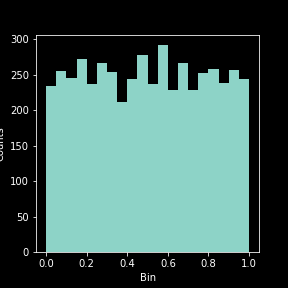
\includegraphics[width=6cm]{random_numbers}
  \caption{Random Generated Samples}
\endminipage\hfill
\minipage{0.5\textwidth}
  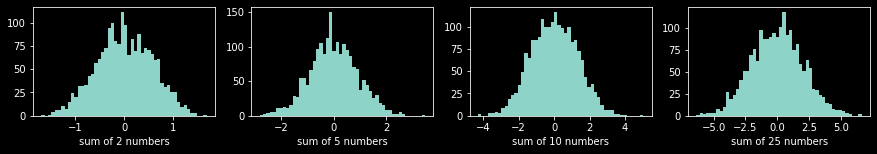
\includegraphics[width=6cm]{sum_random_numbers}
  \caption{Sum of Random Samples}
\endminipage\hfill
\end{figure}

Note that 
\maketitle
\section{Uncertainty in Estimation}

\maketitle
\section{Bivariate Gaussian Distribution}

\maketitle
\section{Sampling for Multivariate Gaussian Distribution}
Data in X is normally distributed with mean = 0 and standard deviation = 1 for both two random variables. This can be observed by the density of data increase when the value come close to 0 and the majority of data is located within 2 standard deviation(-2 to 2).

For Y, although the data also has a normal distribution, the distribution in X-axis is wider than X due to the linear transformation which is performed on X that cause the variance of one random variable to be higher.

\maketitle
\section{Distribution of Projections}
\end{document}